\documentclass[border=8pt]{standalone}
\usepackage{amsmath}
\usepackage{amssymb}
\usepackage{tikz}
\usetikzlibrary{arrows.meta,calc,decorations.pathreplacing,patterns,shapes.geometric,positioning,shadings,plotmarks}

\begin{document}
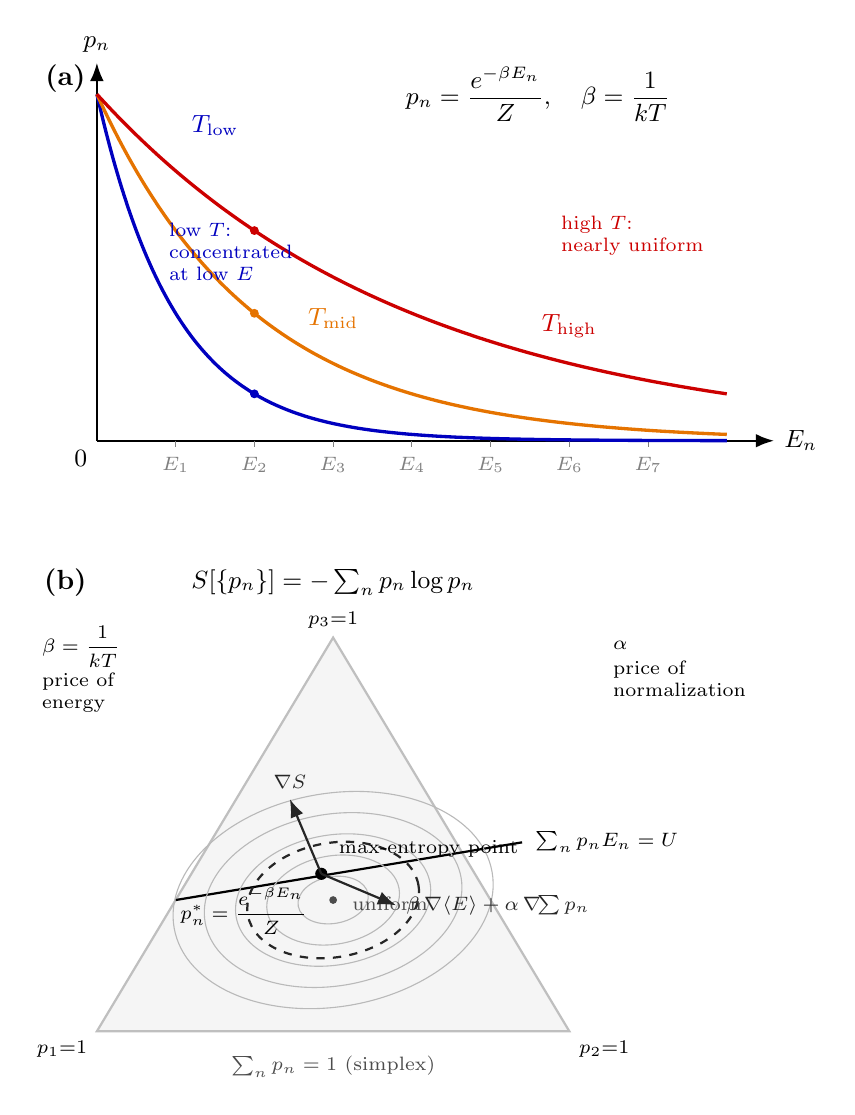
\begin{tikzpicture}[>=Latex]

% =====================================================
% TOP PANEL: Boltzmann distributions at three temperatures
% =====================================================
\begin{scope}[shift={(0,0)}]
  % Axes
  \draw[->, thick] (0,0) -- (8.6,0) node[right] {\small $E_n$};
  \draw[->, thick] (0,0) -- (0,4.8) node[above] {\small $p_n$};

  % Origin label
  \node[below left, font=\small] at (0,0) {$0$};

  % Tick marks on E axis
  \foreach \x/\lab in {1/E_1, 2/E_2, 3/E_3, 4/E_4, 5/E_5, 6/E_6, 7/E_7} {
    \draw[gray] (\x,0) -- (\x,-0.08);
    \node[below, font=\scriptsize, gray] at (\x,-0.08) {$\lab$};
  }

  % Curves: p = A * exp(-beta * E), beta_low : beta_mid : beta_high = 4 : 2 : 1
  % Choose betas so high-T curve is gentlest. T_low < T_mid < T_high => beta_low > beta_mid > beta_high
  % Take beta_low = 1.0, beta_mid = 0.5, beta_high = 0.25
  % Normalize each so amplitude at E=0 is similar visually.

  % Low T (cold, blue): steep
  \draw[blue!75!black, very thick, smooth, samples=80, domain=0:8]
    plot (\x, {4.4*exp(-1.0*\x)});
  \node[blue!75!black, font=\small] at (1.5,4.0) {$T_{\text{low}}$};

  % Mid T (orange): medium
  \draw[orange!90!black, very thick, smooth, samples=80, domain=0:8]
    plot (\x, {4.4*exp(-0.5*\x)});
  \node[orange!90!black, font=\small] at (3.0,1.55) {$T_{\text{mid}}$};

  % High T (red): gentle
  \draw[red!80!black, very thick, smooth, samples=80, domain=0:8]
    plot (\x, {4.4*exp(-0.25*\x)});
  \node[red!80!black, font=\small] at (6.0,1.45) {$T_{\text{high}}$};

  % Sample points at E_n=2 to show ratio
  \fill[blue!75!black] (2,{4.4*exp(-2.0)}) circle (1.6pt);
  \fill[orange!90!black] (2,{4.4*exp(-1.0)}) circle (1.6pt);
  \fill[red!80!black] (2,{4.4*exp(-0.5)}) circle (1.6pt);

  % Title formula
  \node[font=\small] at (5.6,4.4) {$p_n = \dfrac{e^{-\beta E_n}}{Z}, \quad \beta = \dfrac{1}{kT}$};

  % Trend annotations
  \node[font=\scriptsize, blue!75!black, align=left] at (1.7,2.4)
    {low $T$:\\concentrated\\at low $E$};
  \node[font=\scriptsize, red!80!black, align=left] at (6.8,2.6)
    {high $T$:\\nearly uniform};

  % Panel label
  \node[font=\bfseries] at (-0.4,4.6) {(a)};
\end{scope}

% =====================================================
% BOTTOM PANEL: Lagrange multiplier geometry on simplex
% =====================================================
\begin{scope}[shift={(0,-7.5)}]

  % Probability simplex (triangle: p1+p2+p3 = 1, projected)
  % Vertices
  \coordinate (V1) at (0,0);
  \coordinate (V2) at (6,0);
  \coordinate (V3) at (3,5.0);

  % Filled simplex
  \fill[gray!8] (V1) -- (V2) -- (V3) -- cycle;
  \draw[thick, gray!50] (V1) -- (V2) -- (V3) -- cycle;

  % Vertex labels
  \node[below left, font=\scriptsize] at (V1) {$p_1{=}1$};
  \node[below right, font=\scriptsize] at (V2) {$p_2{=}1$};
  \node[above, font=\scriptsize] at (V3) {$p_3{=}1$};

  % Centroid (uniform distribution, MaxEnt without energy constraint)
  \coordinate (C) at (3,1.667);

  % Energy constraint line: <E> = U => crosses simplex as a chord
  % Choose a chord that does not pass through centroid (since U != mean energy under uniform in general)
  \coordinate (EA) at (1.0,1.667);
  \coordinate (EB) at (5.4,2.40);
  \draw[thick, black] (EA) -- (EB);
  \node[font=\scriptsize, anchor=west] at (5.45,2.40) {$\sum_n p_n E_n = U$};

  % Normalization "plane" is the simplex itself; label it
  \node[font=\scriptsize, gray!60!black] at (3.0,-0.45) {$\sum_n p_n = 1$ (simplex)};

  % Tangent / max-entropy point on the chord
  \coordinate (M) at (2.85,2.0);

  % Entropy level curves (concentric ellipses around the centroid C)
  % Drawn as nested ellipses with gradually increasing semi-axes
  \foreach \r in {0.45, 0.85, 1.25, 1.65, 2.05} {
    \draw[gray!55, thin] (C) ellipse [x radius=\r, y radius={0.66*\r}, rotate=10];
  }

  % Highlight the level curve tangent to the constraint at M
  \draw[gray!30!black, thick, dashed] (C) ellipse [x radius=1.1, y radius={0.66*1.1}, rotate=10];

  % Tangency point
  \fill[black] (M) circle (2.2pt);
  \node[font=\scriptsize, anchor=south west] at ($(M)+(0.10,0.08)$) {max-entropy point};
  \node[font=\scriptsize, anchor=north east] at ($(M)+(-0.05,-0.05)$) {$p_n^\ast = \dfrac{e^{-\beta E_n}}{Z}$};

  % Centroid mark
  \fill[gray!60!black] (C) circle (1.4pt);
  \node[font=\scriptsize, gray!60!black, anchor=west] at ($(C)+(0.12,-0.05)$) {uniform};

  % Gradient arrows to indicate Lagrange condition: nabla S parallel to nabla(constraint)
  \draw[->, thick, gray!30!black] (M) -- ($(M)+(-0.40,0.95)$)
    node[anchor=south, font=\scriptsize] {$\nabla S$};
  \draw[->, thick, gray!30!black] (M) -- ($(M)+(0.95,-0.40)$)
    node[anchor=west, font=\scriptsize] {$\beta\,\nabla\langle E\rangle + \alpha\,\nabla\!\!\sum p_n$};

  % Top label: Shannon entropy
  \node[font=\small] at (3.0,5.7) {$S[\{p_n\}] = -\sum_n p_n \log p_n$};

  % Lagrange multiplier reading
  \node[font=\scriptsize, align=left] at (-0.2,4.6)
    {$\beta = \dfrac{1}{kT}$\\[1pt] price of\\ energy};
  \node[font=\scriptsize, align=left] at (7.4,4.6)
    {$\alpha$\\[1pt] price of\\ normalization};

  % Panel label
  \node[font=\bfseries] at (-0.4,5.7) {(b)};
\end{scope}

\end{tikzpicture}
\end{document}
